\documentclass{article}

% Beginn des Headers mit documentclass
\documentclass[bibliography=totocnumbered,ngerman]{scrartcl}
% scrartcl - Artikelformat der KOMA-Klasse
% bibliography=totocnumbered - Literaturverzeichnis wird in das Inhaltsverzeichnis aufgenommen
% ngerman - Für das Dokument wird die Sprache "Deutsch" eingestellt. Damit wird u.a. in SIUnitX die Bereichsangabe mit "bis" statt "to" geschrieben.

% Direkte Angabe von Umlauten im Dokument
\usepackage[utf8]{inputenc}

% Deutsche Sprachanpassungen
\usepackage[ngerman]{babel}

% Erweiterung des Mathe-Satzes (u.a. align-Umgebungen)
\usepackage{amsmath}

% zusätzliche mathematische Symbole (enthält amssymb)
\usepackage{amsfonts}

% Einbinden von Bildern
\usepackage{graphicx}

% Positionierung von Bildern, Tabellen, ...
\usepackage{float}

% Paket für SI-Einheiten
\usepackage{siunitx}
\sisetup{locale = DE}

% Literaturverzeichnis

%% Layout des Literaturverzeichnisses
\usepackage[autostyle]{csquotes}
\bibliographystyle{ieeetr}


% ALTERNATIVE ZU biblatex:
\usepackage[german]{babelbib}

% Zum Einfügen von URLs (hier benötigt fürs Literaturverzeichnis in Zsh mit babelbib)
\usepackage{url}


% Neuer definierter Befehl für Kapitälchen in Überschriften
\newcommand{\textSC}[1]{{\normalfont  \textsc{#1}}}


\usepackage{subcaption}

\begin{document}
    % Wir wollen drei Bilder in einer Figure-Umgebung haben. Zwei sollen nebeneinander sein, das dritte darunter. Das Modul für ein Bild ist ähnlich der figure:

    
    % \begin{subfigure}[<Position>]{<Breite>}
    %     \centering
    %     \includegraphics[width=<Breite>]{<Dateiname>}
    %     \caption{<Beschreibung>}
    %     \label{fig:<Label>}
    % \end{subfigure}

    % ==> Dieses Modul setzen wir nun in eine figure ein. Für die Breiten der zwei Bilder nebeneinander:


    %           0.4\textwidth             0.4\textwidth
    % |-------------------------|    |-------------------------|
    % ----------------------------------------------------------

    % ===> Für das Bild darunter:
    %                         1\textwidth
    % |----------------------------------------------------------|
    %  ----------------------------------------------------------
    % 

    % ... also die gesamte Textbreite. Damit haben wir:

    \begin{figure}[H]
        \centering
        %
        % Einfügen des ersten Bildes:
        %
        %                    oben bestimmt
        %                    vvvvvvvvvvvv
        \begin{subfigure}[b]{0.4\textwidth}
        %                 ^
        %               b = bottom
        %                 = Bild wird unten ausgerichtet
            \centering
            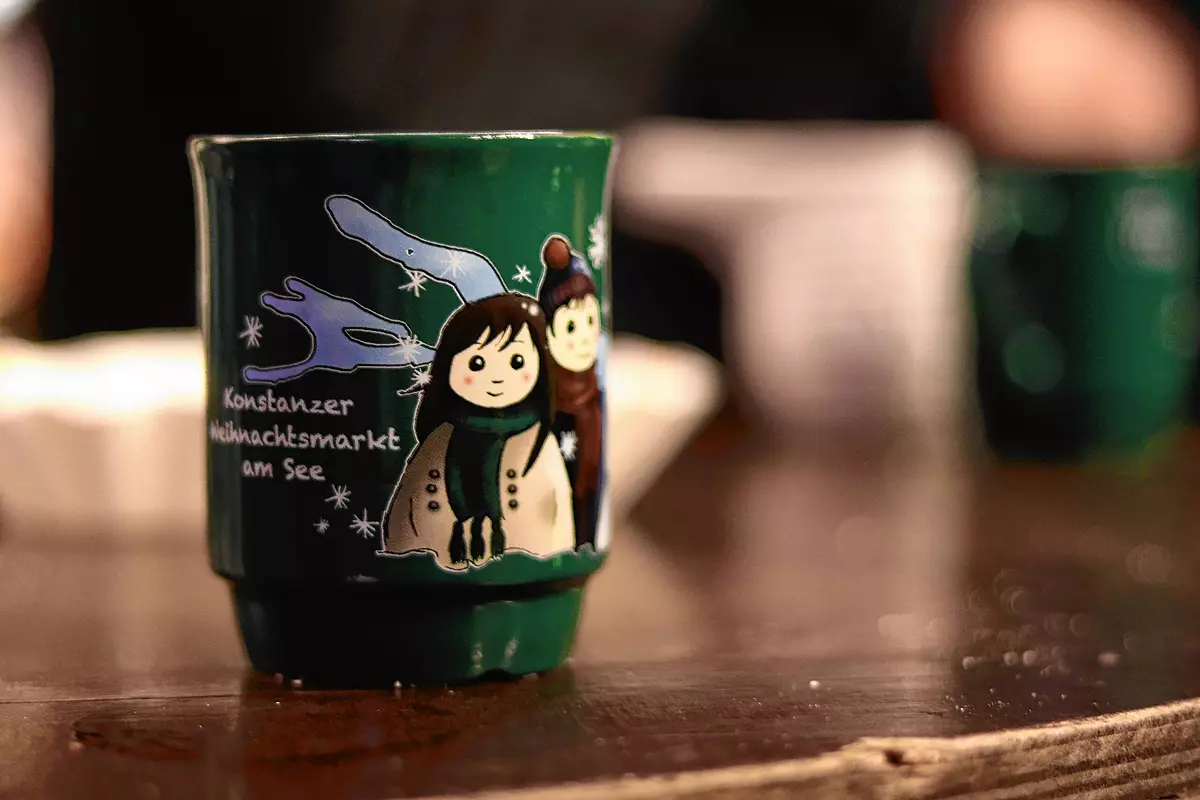
\includegraphics[width=4.5cm]{Bilder/1.png}
            \caption{Bild 1}
            \label{subfig:1} % <== Das Label muss innerhalb der subfigure-Umgebung stehen!
        \end{subfigure}
        % Sofort Bild 2 hinterher:
        \begin{subfigure}[b]{0.4\textwidth}
            \centering
            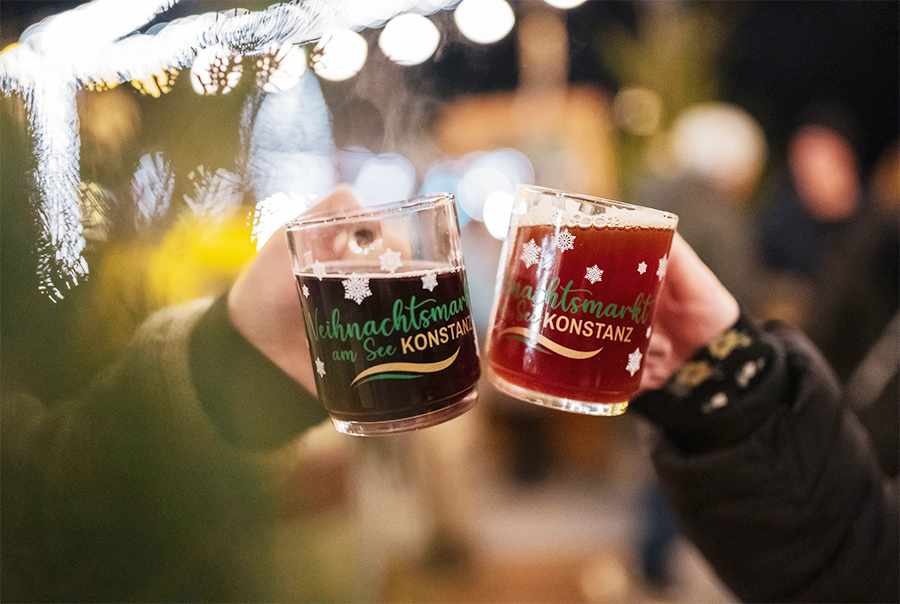
\includegraphics[width=4.5cm]{Bilder/2.png}
            \caption{Bild 2}
            \label{subfig:2}
        \end{subfigure}
        % Und nun das dritte Bild:
        %                   dieses mal anders
        %                    vvvvvvvvvv
        \begin{subfigure}[b]{\textwidth}
            \centering
            \includegraphics[width=10cm]{Bilder/3.png}
            \caption{Bild 3}
            \label{subfig:3}
        \end{subfigure}
        % 
        % Fertig! Caption einbauen, Label für figure setzen und schließen:
        %
        \caption{Drei Bilder nebeneinander}
        \label{fig:3bilder}
    \end{figure}


    % ----------------------------------------------------------------------------------------
    % Aufgabe: 
    %   Sucht euch drei Bilder aus dem Internet und rekreiert das Muster:
    %   
    %   ------------------------------------------------------------------
    %   |                                                                |
    %   |                                                                |
    %   |                                                                |
    %   |                                                                |
    %   |                                                                |
    %   |                                                                |
    %   |                                                                |
    %   |                                                                |
    %   |                                                                |
    %   |                                                                |
    %   |                                                                |
    %   |                                                                |
    %   |                                                                |
    %   ------------------------------------------------------------------
    %   |                               ||                               |
    %   |                               ||                               |
    %   |                               ||                               |
    %   |                               ||                               |
    %   |                               ||                               |
    %   |                               ||                               |
    %   |                               ||                               |
    %   |                               ||                               |
    %   |                               ||                               |
    %   |                               ||                               |
    %   --------------------------------  --------------------------------
    


\end{document}